\documentclass{article}


\usepackage{arxiv}
\usepackage[utf8]{inputenc} % allow utf-8 input
\usepackage[T1]{fontenc}    % use 8-bit T1 fonts
\usepackage{hyperref}       % hyperlinks
\usepackage{url}            % simple URL typesetting
\usepackage{booktabs}       % professional-quality tables
\usepackage{amsfonts}       % blackboard math symbols
\usepackage{nicefrac}       % compact symbols for 1/2, etc.
\usepackage{microtype}      % microtypography
\usepackage{lipsum}
\usepackage{graphicx} 		% Used for Figures

\title{Deep Learning Project: GAN Artwork}


\author{
	Kevin Steele \\
	Department of Electrical Engineering \\
	University of Iowa\\
	\texttt{kevin-steele@uiowa.edu} \\
	%% examples of more authors
	\And
	Brain Fiegel \\
	Department of Industrial and Mechanical Engineering \\
	University of Iowa\\
	\texttt{brian-fiegel@uiowa.edu} \\
	\And
	Stjepan Fiolic \\
	Department of Electrical Engineering \\
	University of Iowa\\
	\texttt{stjepan-fiolic@uiowa.edu} \\
}

\begin{document}
	\maketitle
	
	\begin{abstract}
		https://www.overleaf.com/latex/templates/style-and-template-for-preprints-arxiv-bio-arxiv/fxsnsrzpnvwc
		The Iowa Neuroscience Institute has a desire for a landscape generation process by which DNA sequences are converted to landscape images. Our project is to train a Generative Adversarial Network (GAN) to accomplish this task.
	\end{abstract}
	
	
	% keywords can be removed
	\keywords{Deep Learning \and GAN}
	
	
	\section{Introduction}

	
	This project will create artworks using the DNA sequence of a person as a seed. A generative adversarial network (GAN) will be trained on images of landscape paintings and be tuned to produce a customized artwork for each different DNA sequence. If successful, the algorithm will be deployed at the Iowa Neuroscience Institute to create souvenirs for research subjects.
	
	Testing
	
	\section{Related Works (Optional)}
	\label{sec:headings}
	
	\begin{itemize}
		\item If you find it necessary to have a separate section to deep dive into other relevant works in literature, create a section titled "Related Work".
		\item Try to categorize your/other people's previous works and build a *story*. Don't just list some facts. The worst thing to do is something like: "Smith et al. did this. Johnson et al. did that. Xu et al. did this. ..." ----a simple listing of papers. Instead, tell a story (like a fun history book).
		\item For the scope of this project, it is not always necessary.
		\item If you plan to transform this course project into a journal/conference submission, it should be helpful to have it written up.
	\end{itemize}
	
	See Section \ref{sec:headings}.
	
	
	\section{Problem Definition}
	\label{sec:problemdef}
	Our goal is to convert a valid DNA input sequence into a landscape image using a Generative Adversarial Network (GAN). Examples of these can be seen in the Data section \ref{sec:data}. This is a Text-to-Image synthesis issue, with the generator taking valid DNA codons (TCAG) as input and creating landscape 224 by 224 by 3 (RBG) images as output. Image values range within [0,255] across the 3 color channels. Similar to a more general Text-to-Image GAN, which would take text descriptions to generate images, the DNA codon sequence will be a translated language by which we generate landscapes. Valid DNA codons follow the standard generic code table with valid inputs of T, C, A, and G in groups of 3. Each sequence must also start with a start codon and end with an end codon. Noted in the original table, there are 25 different amino acids that these codons correspond to. While it is not currently our goal, this fact could be used similarly to an alphabet, and thusly a sentence or description of the image. 

	Looking more comprehensively at the GAN, the generator takes as input valid codon, considered the latent space of the system, and outputs the image we desire. The discriminator would take as input an image, either directly from the dataset or from the generator, and return the probability that the image is real (direct input) or fake (generated input). It is obvious that, generally, DNA does not map to images in the real world. In this case, we have a set of unmapped inputs to model, which will require a specialized GAN architecture. A few architectures have been proposed in this realm, particularly StackGAN \cite{zhang2017stackgan} for text-to-image and CycleGAN \cite{CycleGAN2017} for unpaired image mapping (though the principle works for text). This involves mapping encoded text to image feature maps generated by the generator, then do the reverse with an image encoder. A more recent attempt at this is MirrorGAN \cite{qiao2019mirrorgan}.  
	
	For our purposes, we currently create input to the generator, the latent variables, by converting the DNA sequence to a normalized average value between [0, 1]. Thus, we convert the variable length string into a single floating-point feature. We also have plans to test using an Auto-Encoder to create this latent variable, as it works as a trainable solution. 

	
	\section{Data}
	\label{sec:data}
	The datasets used within this project are a Landscape dataset obtained from Kaggle and a DNA dataset obtained from Joint Research Center. They can be found at their respective pages:
	\begin{center}
		\url{https://www.kaggle.com/arnaud58/landscape-pictures} \\
		\url{https://data.jrc.ec.europa.eu/dataset/2abb5c2b-3ab6-4ce4-b103-cb1c5fc7349e}
	\end{center}

	\subsection{Landscape Dataset}
	The landscape dataset contains a variety of non-descriptive landscape images. There are no classifications or metadata for any image. All images start as JPEG images of varying sizes, but are pre-processed to be 224-224, as can be seen in Figure \ref{fig:landscapes}. The images used were scraped from Flickr images
	
	\begin{figure}[h]
		\centering
		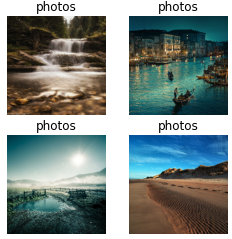
\includegraphics[scale=1]{images/landscapes}
		\caption{Pre-processed images}
		\label{fig:landscapes}
	\end{figure}

	
	\subsection{DNA Dataset}
	The DNA dataset contains various sequences of DNA codons. Collected by the Joint Research Center by sequencing genetically modified strains of bacillus subtilis used for production of vitamin B2 in feed additive. \\
	Data is formatted in a {\em .fastq} file with the structure found in Table \ref{tab:dna}.
	
	\begin{table}
		\caption{DNA Formatting}
		\centering
		\begin{tabular}{llllll}
			\toprule
			ID     & Name     & Description & Number of Features & Per letter annotation for: & Sequence \\
			\bottomrule
		\end{tabular}
		\label{tab:dna}
	\end{table}
	
	\bibliographystyle{unsrt}  
	%\bibliography{references}  %%% Remove comment to use the external .bib file (using bibtex).
	%%% and comment out the ``thebibliography'' section.
	
	
	%%% Comment out this section when you \bibliography{references} is enabled.
	\begin{thebibliography}{1}
		\bibitem{zhang2017stackgan}
		Han Zhang, Tao Xu, Hongsheng Li, Shaoting Zhang, Xiaogang Wang, Xiaolei Huang, and 
		Dimitris Metaxas.
		\newblock StackGAN: Text to Photo-realistic Image Synthesis with Stacked 
		Generative Adversarial Networks.
		\newblock {\em arXiv preprint arXiv:1612.03242}, 2017.
		

		\bibitem{CycleGAN2017}
		Zhu, Jun-Yan and Park, Taesung and Isola, Phillip and Efros, Alexei A.
		\newblock Unpaired Image-to-Image Translation using Cycle-Consistent Adversarial Networks.
		\newblock In IEEE International Conference on Computer Vision (ICCV), 2017.

		
		\bibitem{qiao2019mirrorgan}
		Tingting Qiao and Jing Zhang and Duanqing Xu and Dacheng Tao.
		\newblock MirrorGAN: Learning Text-to-image Generation by Redescription
		\newblock {\em arXiv preprint arXiv:1903.05854}, 2019.
		
	\end{thebibliography}
	
	
\end{document}